\documentclass[10,a4paperpaper,]{article}

  \title{Replication Report for MacKinnon, Lockwood, and Williams (2004)}
  \author{Tristan Tibbe\textsuperscript{1} \and Amanda Montoya\textsuperscript{2}}
  \date{%
		\textsuperscript{1} University of California, Los Angeles\\%
		\textsuperscript{2} University of California, Los Angeles~\\[2ex]
		\today
   }
  


\newcommand{\iblue}{008080}
\newcommand{\igray}{d4dbde}
\usepackage{pdflscape}
\newcommand{\blandscape}{\begin{landscape}}
\newcommand{\elandscape}{\end{landscape}}

% Author: Karol KozioL
% License: GPL-3
% Modified by: Sarah Wagner & Anna Lohmann

% % % packages -----------------------------------------------------------------------------------
\usepackage{amsmath}
\usepackage{array}
\usepackage{booktabs}
\usepackage{calc}
\usepackage{eso-pic}
\usepackage{fancyhdr}
\usepackage{fontspec}
\usepackage[left = 2.5cm, right = 2.5cm, top = 1.2cm, bottom = 1.2cm, includeheadfoot]{geometry}
\usepackage{graphicx}
\usepackage[utf8]{inputenc}
\usepackage{lastpage}
\usepackage{multirow}
\usepackage{tabularx} 
\usepackage{tikz}
\usepackage{titlesec}
\usepackage{xcolor, colortbl}
\usepackage{url} 
\usepackage[hidelinks]{hyperref} 
\usepackage{pmboxdraw}
\usepackage{placeins}
\usepackage{enumitem}
\usepackage{longtable}
\usepackage{lscape}
%\usepackage{verbatim}
%\makeatletter
%\def\verbatim@font{\scriptsize\ttfamily}
%\makeatother
%\RequirePackage[normalem]{ulem} %DIF PREAMBLE
%\RequirePackage{color}
%\providecommand{\tightlist}{%
%	\setlength{\itemsep}{0pt}\setlength{\parskip{0pt}}
\providecommand{\tightlist}{%
  \setlength{\itemsep}{0pt}\setlength{\parskip}{0pt}}
% % % settings -----------------------------------------------------------------------------------

% % custom colors
\definecolor{iblue}{HTML}{\iblue}
\definecolor{igray}{HTML}{\igray}

% definition of pagename
\newcommand\pagename{Page}

% % fonts 
\defaultfontfeatures{Mapping = tex-text}
\setmainfont[BoldFont = Lato-Bold.ttf, ItalicFont = Lato-Italic.ttf, BoldItalicFont = Lato-BoldItalic.ttf]{Lato-Regular.ttf}
\newfontfamily\headingfont[ItalicFont = Lato-BlackItalic.ttf]{Lato-Black.ttf}
%\setmonofont{Ubuntu Mono}
\setmonofont[Scale=0.90,
BoldFont=UbuntuMono-Bold.ttf,
%ItalicFont=UbuntuMono-Italic.ttf,
BoldItalicFont=UbuntuMono-BoldItalic.ttf
]{UbuntuMono-Regular.ttf}

\makeatletter
\def\verbatim@font{\linespread{1}\normalfont\ttfamily}
\makeatother

% % sections
\titleformat{\section}{\color{iblue}\headingfont\Large\bfseries}{\thesection}{1em}{}[\titlerule]
\titleformat{\subsection}{\color{iblue}\headingfont\large\bfseries}{\thesubsection}{1em}{}
\titleformat{\subsubsection}{\color{iblue}\headingfont\bfseries}{\thesubsubsection}{1em}{}

% % misc
\setlength{\parindent}{0em} 
\linespread{1.5}
\raggedright
\newcolumntype{C}{>{\centering\arraybackslash}X}


\makeatletter

% pagestyle titlepage
\fancypagestyle{customtitle}{
	\lhead{}
	\chead{}
	\rhead{}
	\makeatother
	\lfoot{}
	\cfoot{}
	\rfoot{}
}




% % % header and footer ---------------------------------------------------------------------------
\pagestyle{fancy}
\lhead{}
\chead{}
\rhead{}
\makeatother
\newlength{\myheight}
\lfoot{}
\cfoot{}
\rfoot{\pagename~\thepage \hspace{1pt} / \pageref{LastPage}}
\renewcommand\headrulewidth{0pt}
\renewcommand\footrulewidth{0pt}




\begin{document}


\renewcommand{\contentsname}{Table of Contents}

\renewcommand{\pagename}{Page}


\urlstyle{same}

\maketitle 

\subsection*{Abstract}

We attempted to replicate two simulation studies conducted by MacKinnon,
Lockwood, and Williams (2004) comparing different methods of
constructing confidence intervals for the indirect effect in mediation
analysis. The first study compared the performance of normal theory
confidence intervals to confidence intervals based on the distribution
of the product of two normally distributed independent random variables.
The second study compared these two confidence interval methods to
resampling methods of computing confidence intervals, including the
percentile bootstrap, the bias-corrected bootstrap, the jackknife, the
bootstrap-\(t\), the bootstrap-\(Q\), and Monte Carlo confidence
intervals. The overall conclusions of the original article (i.e., that
the distribution of the product and resampling confidence intervals
performed better than the normal theory confidence interval) were
replicated in our study, but there were still many discrepancies between
our results and the original results. \vskip 2em

\noindent\makebox[\textwidth]{\large Correspondence concerning this replication report should be addressed to:}\par
\noindent\makebox[\textwidth]{\large tibbe1td@g.ucla.edu}\par

\clearpage

\section{Introduction}

This replication report documents the replication attempt of the
simulation study MacKinnon, D. P., Lockwood, C. M., \& Williams, J.
(2004). Confidence limits for the indirect effect: Distribution of the
product and resampling methods. \emph{Multivariate Behavioral Research,
39}, 99 - 128. Following the definition of Rougier et al. (2017) we
understand the replication of a published study as writing and running
new code based on the description provided in the original publication
with the aim of obtaining the same results.

\section{Method}

\subsection{Information basis}

To complete this replication attempt, we utilized information from (1)
the original article by MacKinnon, Lockwood, and Williams (2004), (2)
additional information in a book by Manly (1997), and (3) an R function
in a package introduced in Tofighi and MacKinnon (2011).

\subsection{Data Generating Mechanism}

Information provided in the above mentioned sources indicated that the
following simulation factors were systematically varied in generating
the artificial data in study 1 and study 2.

\begin{longtable}[]{@{}lll@{}}
\toprule
Study 1: Simulation factor & No. levels & Levels\tabularnewline
\midrule
\endhead
\emph{Varied} & &\tabularnewline
Confidence interval method & 2 & \(z\) method, \(M\)
method\tabularnewline
Sample size & 5 & 50, 100, 200, 500, 1000\tabularnewline
\(\alpha\) effect size & 4 & 0, .14, .39, .59\tabularnewline
\(\beta\) effect size & 4 & 0, .14, .39, .59\tabularnewline
\emph{Fixed} & &\tabularnewline
Direct effect size & & 0\tabularnewline
Intercepts & & 0\tabularnewline
\emph{Randomly Sampled} & &\tabularnewline
\(X\) values & & sampled from \(N(0,1)\)\tabularnewline
Error terms & & sampled from \(N(0,1)\)\tabularnewline
\bottomrule
\end{longtable}

\begin{longtable}[]{@{}lll@{}}
\toprule
\begin{minipage}[b]{0.18\columnwidth}\raggedright\strut
Study 2: Simulation factor\strut
\end{minipage} & \begin{minipage}[b]{0.05\columnwidth}\raggedright\strut
No. levels\strut
\end{minipage} & \begin{minipage}[b]{0.37\columnwidth}\raggedright\strut
Levels\strut
\end{minipage}\tabularnewline
\midrule
\endhead
\begin{minipage}[t]{0.18\columnwidth}\raggedright\strut
\emph{Varied}\strut
\end{minipage} & \begin{minipage}[t]{0.05\columnwidth}\raggedright\strut
\strut
\end{minipage} & \begin{minipage}[t]{0.37\columnwidth}\raggedright\strut
\strut
\end{minipage}\tabularnewline
\begin{minipage}[t]{0.18\columnwidth}\raggedright\strut
Confidence interval method\strut
\end{minipage} & \begin{minipage}[t]{0.05\columnwidth}\raggedright\strut
9\strut
\end{minipage} & \begin{minipage}[t]{0.37\columnwidth}\raggedright\strut
\(z\) method, \(M\) method, empirical-\(M\) method, jackknife,
percentile bootstrap, bias-corrected bootstrap, bootstrap-\(t\),
bootstrap-\(Q\), Monte Carlo method\strut
\end{minipage}\tabularnewline
\begin{minipage}[t]{0.18\columnwidth}\raggedright\strut
Sample size\strut
\end{minipage} & \begin{minipage}[t]{0.05\columnwidth}\raggedright\strut
4\strut
\end{minipage} & \begin{minipage}[t]{0.37\columnwidth}\raggedright\strut
25, 50, 100, 200\strut
\end{minipage}\tabularnewline
\begin{minipage}[t]{0.18\columnwidth}\raggedright\strut
\(\alpha\) effect size\strut
\end{minipage} & \begin{minipage}[t]{0.05\columnwidth}\raggedright\strut
4\strut
\end{minipage} & \begin{minipage}[t]{0.37\columnwidth}\raggedright\strut
0, .14, .39, .59\strut
\end{minipage}\tabularnewline
\begin{minipage}[t]{0.18\columnwidth}\raggedright\strut
\(\beta\) effect size\strut
\end{minipage} & \begin{minipage}[t]{0.05\columnwidth}\raggedright\strut
4\strut
\end{minipage} & \begin{minipage}[t]{0.37\columnwidth}\raggedright\strut
0, .14, .39, .59\strut
\end{minipage}\tabularnewline
\begin{minipage}[t]{0.18\columnwidth}\raggedright\strut
Confidence level\strut
\end{minipage} & \begin{minipage}[t]{0.05\columnwidth}\raggedright\strut
3\strut
\end{minipage} & \begin{minipage}[t]{0.37\columnwidth}\raggedright\strut
95\%, 90\%, 80\%\strut
\end{minipage}\tabularnewline
\begin{minipage}[t]{0.18\columnwidth}\raggedright\strut
\emph{Fixed}\strut
\end{minipage} & \begin{minipage}[t]{0.05\columnwidth}\raggedright\strut
\strut
\end{minipage} & \begin{minipage}[t]{0.37\columnwidth}\raggedright\strut
\strut
\end{minipage}\tabularnewline
\begin{minipage}[t]{0.18\columnwidth}\raggedright\strut
Direct effect size\strut
\end{minipage} & \begin{minipage}[t]{0.05\columnwidth}\raggedright\strut
\strut
\end{minipage} & \begin{minipage}[t]{0.37\columnwidth}\raggedright\strut
0\strut
\end{minipage}\tabularnewline
\begin{minipage}[t]{0.18\columnwidth}\raggedright\strut
Intercepts\strut
\end{minipage} & \begin{minipage}[t]{0.05\columnwidth}\raggedright\strut
\strut
\end{minipage} & \begin{minipage}[t]{0.37\columnwidth}\raggedright\strut
0\strut
\end{minipage}\tabularnewline
\begin{minipage}[t]{0.18\columnwidth}\raggedright\strut
\emph{Randomly Sampled}\strut
\end{minipage} & \begin{minipage}[t]{0.05\columnwidth}\raggedright\strut
\strut
\end{minipage} & \begin{minipage}[t]{0.37\columnwidth}\raggedright\strut
\strut
\end{minipage}\tabularnewline
\begin{minipage}[t]{0.18\columnwidth}\raggedright\strut
\(X\) values\strut
\end{minipage} & \begin{minipage}[t]{0.05\columnwidth}\raggedright\strut
\strut
\end{minipage} & \begin{minipage}[t]{0.37\columnwidth}\raggedright\strut
sampled from \(N(0,1)\)\strut
\end{minipage}\tabularnewline
\begin{minipage}[t]{0.18\columnwidth}\raggedright\strut
Error terms\strut
\end{minipage} & \begin{minipage}[t]{0.05\columnwidth}\raggedright\strut
\strut
\end{minipage} & \begin{minipage}[t]{0.37\columnwidth}\raggedright\strut
sampled from \(N(0,1)\)\strut
\end{minipage}\tabularnewline
\bottomrule
\end{longtable}

\subsubsection{Sample size}

Study 1 in the original article generated sample sizes of 50, 100, 200,
500, and 1000. For the second study, \emph{``Because resampling methods
are particularly useful when sample sizes are small, the two largest
sample sizes from Study 1 were dropped and a sample size of 25 was
added''} (original article, p.~8), resulting in sample sizes of 25, 50,
100, and 200.

\subsubsection{$\alpha$ and $\beta$ effect sizes}

Both studies in the original article generated \(\alpha\) and \(\beta\)
effect sizes of 0, .14, .39, and .59, which \emph{``corresponded to
zero, small (2\% of the variance), medium (13\% of the variance), and
large (26\% of the variance) effect sizes as described in Cohen (1988,
p.~412-414)''} (original article, p.~6). In study 1, every permutation
of the \(\alpha\) and \(\beta\) values were multiplied together to form
a total of 16 population indirect effects \(\alpha \beta\). In study 2,
\emph{``to reduce the considerable computational demands of simulation
studies of resampling methods''} (original article, p.~8), only ten of
these permutations were generated: \(\alpha = 0\) with \(\beta = 0\),
\(\alpha = 0\) with \(\beta = .14\), \(\alpha = 0\) with
\(\beta = .39\), \(\alpha = 0\) with \(\beta = .59\), \(\alpha = .14\)
with \(\beta = .14\), \(\alpha = .39\) with \(\beta = .39\),
\(\alpha = .59\) with \(\beta = .59\), \(\alpha = .14\) with
\(\beta = .39\), \(\alpha = .14\) with \(\beta = .59\), and
\(\alpha = .39\) with \(\beta = .59\).

\subsubsection{Confidence level}

In study 1, the confidence level of the confidence intervals was fixed
at 95\%. In study 2, the confidence level of the confidence intervals
generated for the indirect effect were varied from 95\%, to 90\%, to
80\% so that the proportion of times the true indirect effect fell to
the left and the right of the confidence intervals could be calculated
for different confidence levels.

\subsubsection{Repititions}

In study 1, each of the 16 indirect effects \(\times\) 5 sample sizes =
80 conditions was repeated 10000 times (original article, p.~6). In
study 2, each of the 10 indirect effects \(\times\) 4 sample sizes = 40
conditions was repeated 1000 times. In addition, for the bootstrap
methods in study 2, 1000 bootstrap samples were drawn from the generated
sample in each of the 1000 iterations of each of the 40 conditions
(original article, p.~8).

\subsubsection{Data Generating Process}

To generate \(a\) and \(b\), the sample estimates of \(\alpha\) and
\(\beta\), sample values of \(M\) and \(Y\) were first generated using
the equations: \[M = i_{01} + \alpha X + \varepsilon_1\]
\[Y = i_{02} + c'X + \beta M + \varepsilon_2\] where \(X\) was the
independent variable, \(M\) was the mediator variable, \(Y\) was the
outcome variable, the \(i_0\) terms were the intercepts, \(c'\) was the
direct effect, and the \(\varepsilon\)s were the error terms. The
intercepts and the direct effect were set to zero, so the equations
simplified to:

\begin{gather} 
M = \alpha X + \varepsilon_1 \\
Y = \beta M + \varepsilon_2  
\end{gather}

After generating \(M\) and \(Y\) values, \(a\) was then calculated using
the following equation:
\[\mathbf{a} = (\mathbf{X_{dm}}^T \mathbf{X_{dm}})^{-1}\mathbf{X_{dm}}^T\mathbf{m}\]
where \(\mathbf{a}\) is a column vector containing the ordinary least
squares estimates of the intercept and \(\alpha\) (i.e., \(a\)),
\(\mathbf{X_{dm}}\) is a design matrix formed by combining a column of
ones and a column containing the values of \(X\), and \(\mathbf{m}\) is
a column vector containing the values of \(M\). Finally, \(a\) was
extracted from \(\mathbf{a}\).

Similarly, \(b\) was calculated using the following equation:

\[\mathbf{b} = (\mathbf{M_{dm}}^T \mathbf{M_{dm}})^{-1}\mathbf{M_{dm}}^T\mathbf{y}\]
where \(\mathbf{b}\) is a column vector containing the ordinary least
squares estimates of the intercept, the direct effect, and \(\beta\)
(i.e., \(b\)); \(\mathbf{M_{dm}}\) is a design matrix formed by
combining a column of ones, a column containing the values of \(X\), and
a column containing the values of \(M\); and \(\mathbf{y}\) is a column
vector containing the values of \(Y\). Finally, \(b\) was extracted from
\(\mathbf{b}\).

\begin{minipage}{\linewidth}
Data generation for study 1 (and study 2) can be summarized with the following pseudo code:

\texttt{For 10000 (1000 for study 2) repetitions of each of 80 (40 for study 2) unique conditions:}
\begin{itemize}[leftmargin=*] 
    \item[--] \texttt{Sample number of $X$ values determined by sample size from standard normal distribution.}
    \item[--] \texttt{Use Equation 1 with $\varepsilon_1$ sampled from standard normal distribution to generate $M$.}
    \item[--] \texttt{Use Equation 2 with $\varepsilon_2$ sampled from standard normal distribution to generate $Y$.}
    \item[--] \texttt{Solve Equations 1 and 2 to find the ordinary least squares estimators of $\alpha$ (i.e., $a$) and $\beta$ (i.e., $b$) and estimates of their standard errors.}
\end{itemize}
\end{minipage}

\subsection{Compared Methods}

Study 1 compared two methods of generating confidence intervals for the
indirect effect in simple mediation analysis. The first is the normal
(\(z\)) method where the indirect effect is assumed to be normally
distributed and a typical 95\% confidence interval is calculated around
the indirect effect using a z-score critical value. The second is the
distribution of the product (\(M\)) method, which uses the distribution
of the product of two independent normally distributed random variables
to find critical values for a confidence interval for the indirect
effect.

In addition to the \(z\) and \(M\) methods, study 2 compared an
additional seven methods of creating confidence intervals for the
indirect effect. These included an alternate distribution of the product
method (referred to in the original article as the ``empirical-\(M\)''
method, p.~9), the jackknife, the percentile bootstrap, the
bias-corrected bootstrap, the bootstrap-\(t\), the bootstrap-\(Q\), and
the Monte Carlo methods of generating confidence intervals. Also in
study 2, 95\%, 90\%, and 80\% confidence intervals were formed for each
method.

\subsubsection{$z$ method}

Confidence intervals were generated using the equation
\(ab \pm z_{1- \omega/2} \times \hat{\sigma}_{ab}\) where \(ab\) is the
sample indirect effect, \(z_{1- \omega/2}\) is the z-score corresponding
to \(1- \omega/2 \times 100\) percentile of the normal distribution
(\(\omega\) = alpha level determined by confidence level set), and
\(\hat{\sigma}_{ab}\) is the estimated standard error of the sample
indirect effect calculated using the equation
\(\hat{\sigma}_{ab} = a^2 \hat{\sigma}^2_b + b^2 \hat{\sigma}^2_a\) (see
p.~3 of original article).

\subsubsection{$M$ method}

Confidence intervals in study 1 were generated using the equations Upper
Limit \(=ab+\text{Meeker Upper} \times \hat{\sigma}_{ab}\) and Lower
Limit \(=ab+\text{Meeker Lower} \times \hat{\sigma}_{ab}\) (see p.~5 of
original article). The Meeker Upper and Lower values were taken from
tables in Meeker, Cornwell, and Aroian (1981) (see p.~5 of original
article), which gave the percentiles of the distribution of the product
determined by the values of \(\delta_1 = a/\hat{\sigma}_a\) and
\(\delta_2 = b/\hat{\sigma}_b\). Because these tables only provided
values of \(\delta_1\) and \(\delta_2\) in increments of .4, MacKinnon,
Lockwood, and Williams (2004) improved precision in study 2 by utilizing
a FORTRAN algorithm to find percentiles for values of \(\delta_1\) and
\(\delta_2\) in increments of .2 (see p.~9 of original article).

\subsubsection{Empirical-$M$ method}

Confidence intervals were generated using the same equations used in the
\(M\) method, except the Meeker Upper and Meeker Lower values were
replaced with empirical values the authors simulated in case the
theoretical values of the Meeker, Cornwell, and Aroian (1981) tables did
not apply to the indirect effect (see p.~9 of original article).

\subsubsection{Jackknife}

The jackknife involves removing one observation from the dataset and
then calculating the indirect effect estimate based on this new dataset
containing \(n-1\) observations, and then repeating this process for
each observation in the original dataset until a set of \(n\) indirect
effect estimates each based on a dataset containing \(n-1\) observations
is produced. Confidence intervals were generated using the same
equations used in the \(z\) method, except the sample indirect effect
estimate \(ab\) was replaced by the average jackknife indirect effect
estimate (see p.~9 of original article) and the estimated indirect
effect standard error \(\hat{\sigma}_{ab}\) was replaced with the
jackknife estimate of the standard error (see Equation 8 on p.~9 of
original article).

\subsubsection{Percentile Bootstrap}

Bootstrapping involves resampling observations with replacement from the
original sample of \(n\) observations to create new samples of size
\(n\), and then calculating the indirect effect estimate for each of
these bootstrap samples. By collecting many bootstrap samples in this
way, these samples form an empirical sampling distribution of the
indirect effect. The percentile bootstrap confidence interval was then
created using the \(\omega/2 \times 100\) and \(1- \omega/2 \times 100\)
percentiles of this bootstrap sampling distribution as the lower and
upper limits of the confidence interval. For example, a 95\% confidence
interval would set an alpha level of .05, and thus the
\(.05/2 \times 100 = 2.5\)th and the \(1- .05/2 \times 100 = 97.5\)th
percentiles of the bootstrap sampling distribution would be used for the
percentile bootstrap confidence interval.

\subsubsection{Bias-Corrected Bootstrap}

The bias-corrected bootstrap confidence interval involved first creating
the percentile bootstrap confidence interval and then adjusting its
lower and upper limits using the process described on p.~10 of the
original article.

\subsubsection{Bootstrap-$t$}

The bootstrap-\(t\) confidence interval involved generating bootstrap
\(t\)-values rather than bootstrap estimates of the indirect effect, but
the exact method used to generate these \(t\)-values in the article was
unclear and we had to infer what their procedure was for this
replication attempt (see replicator degrees of freedom table below).
Once the \(t\)-values were generated, the lower and upper limits of the
bootstrap-\(t\) confidence interval were found using the formulas
\(ab - t_{1-\omega/2} \times \hat{\sigma}_{ab}\) and
\(ab - t_{\omega/2} \times \hat{\sigma}_{ab}\), respectively, where
\(t_{1-\omega/2}\) and \(t_{\omega/2}\) are the \(1-\omega/2\) and
\(\omega/2\) percentiles of the distribution of \(t\)-values formed.

\subsubsection{Bootstrap-$Q$}

The bootstrap-\(Q\) confidence interval involved transforming the
bootstrap \(t\)-values calculated for the bootstrap-\(t\) confidence
interval using the formula \(Q = t + (st^2)/3 + (s^2t^3)/27 + s/(6N)\),
where \(s\) is the skewness of the distribution of \(t\)-values and
\(N\) is the number of \(t\)-values in the distribution, 1000. The
\(\omega/2\) and \(1-\omega/2\) percentiles of this distribution of
\(Q\)-values were then selected and back-transformed to \(t\)-values
using the formula \(t = 3([1+s(Q - s/(6N))]^{1/3} - 1)/s\) from Manly
(1997). The lower and upper limits of the bootstrap-\(Q\) confidence
interval were then found using the same formula used for the
bootstrap-\(t\) confidence interval. However, the formula used to
calculate the skewness was not provided in the original article, and
thus we had to infer what was used for this replication attempt (see
replicator degrees of freedom table below).

\subsubsection{Monte Carlo method}

The Monte Carlo method involves first taking the original sample
estimates of \(a\), \(b\), and their standard errors \(\hat{\sigma}_a\)
and \(\hat{\sigma}_b\), and using them as mean and standard deviation
parameters to specify normal distributions for \(a\) and \(b\). Next,
\(a\) and \(b\) values are randomly sampled from these normal
distributions and then multiplied to form indirect effect estimates
\(ab\). This process is then repeated many times to produce a sampling
distribution of the indirect effect. The Monte Carlo confidence interval
was then formed using the same procedure used for the percentile
bootstrap confidence interval, taking the \(\omega/2 \times 100\) and
\(1- \omega/2 \times 100\) percentiles of the sampling distribution as
the lower and upper limits of the confidence interval.

\subsection{Performance measures}

In study 1, the performance of the \(z\) method and the \(M\) method
95\% confidence intervals were compared in terms of ``the proportion of
times the true {[}indirect effect{]} value was above the upper
confidence limit and the proportion of times the true value was below
the lower confidence limit'' (original article, p.~6). These proportions
were compared to the proportions expected under the confidence level set
to determine the accuracy of the method. For example, with a 95\%
confidence interval, it would be expected that .025 of the true indirect
effect values would fall above the upper confidence limit and .025 would
fall below the lower confidence limit. The liberal robustness criterion
given in Bradley (1978) was used to determine if each proportion was
robust: If a proportion fell outside the interval \(.5 \times \omega/2\)
to \(1.5 \times \omega/2\) (which equates to .0125 to .0375 for a 95\%
confidence interval), it was considered to be different from the
expected proportion and thus not robust. These proportions were marked
by an asterisk in their data tables.

In study 2, the performance of the \(z\) method, the \(M\) method, the
empirical-\(M\) method, the jackknife, the percentile bootstrap, the
bias-corrected bootstrap, the bootstrap-\(t\), the bootstrap-\(Q\), and
the Monte Carlo method 95\%, 90\%, and 80\% confidence intervals were
compared in terms of accuracy (defined and measured the same way it was
done in study 1), type I error rate, and power. The liberal robustness
criterion given in Bradley (1978) was used to compare type I error
rates: If a type I error rate fell outside the interval
\(.5 \times \omega\) to \(1.5 \times \omega\) (which equates to .025 to
.075 for a 95\% confidence interval), it was marked by an asterisk in
their data tables.

\subsection{Technical implementation}

While the original simulation study was carried out in SAS, our
replication was implemented using the R programming environment (details
regarding software versions can be obtained from the section
Reproducibility Information).

The following table provides an overview of replicator degrees of
freedom, i.e.~decisions that had to be made by the replicators because
of insufficient or contradicting information. Issues were resolved by
discussion among the replicators. Decisions were based on what the
replicators perceived to be the most likely implementation with
likeliness estimated by common practice and/or guideline
recommendations. Wherever feasible multiple interpretations where
implemented.

\begin{longtable}[]{@{}lll@{}}
\toprule
\begin{minipage}[b]{0.30\columnwidth}\raggedright\strut
Issue\strut
\end{minipage} & \begin{minipage}[b]{0.30\columnwidth}\raggedright\strut
Replicator decision\strut
\end{minipage} & \begin{minipage}[b]{0.30\columnwidth}\raggedright\strut
Justification\strut
\end{minipage}\tabularnewline
\midrule
\endhead
\begin{minipage}[t]{0.30\columnwidth}\raggedright\strut
In terms of seeds used, the only information provided in the original
article was that, ``current time {[}was{]} used as the seed for each
simulation'' (pg. 6).\strut
\end{minipage} & \begin{minipage}[t]{0.30\columnwidth}\raggedright\strut
We set the seed to the current time on the clock when we ran each
simulation: 1:19pm=119 for study 1 and 12:00pm=1200 for study 2.\strut
\end{minipage} & \begin{minipage}[t]{0.30\columnwidth}\raggedright\strut
We felt this was following their directions to the best of our
abilities.\strut
\end{minipage}\tabularnewline
\begin{minipage}[t]{0.30\columnwidth}\raggedright\strut
--------------------------------\strut
\end{minipage} & \begin{minipage}[t]{0.30\columnwidth}\raggedright\strut
--------------------------------\strut
\end{minipage} & \begin{minipage}[t]{0.30\columnwidth}\raggedright\strut
--------------------------------\strut
\end{minipage}\tabularnewline
\begin{minipage}[t]{0.30\columnwidth}\raggedright\strut
No explanation of how values from Meeker, Cornwell, and Aroian (1981)
tables were implemented for \(M\) method in study 1. It was also not
explained how FORTRAN algorithm was implemented in study 2. See
subsection 2.6 for more information.\strut
\end{minipage} & \begin{minipage}[t]{0.30\columnwidth}\raggedright\strut
We used the \texttt{medci} R function from the RMediation package
created by Tofighi and MacKinnon (2011) to produce critical values for
\(M\) method in both studies 1 and 2. See subsection 2.6 for more
information.\strut
\end{minipage} & \begin{minipage}[t]{0.30\columnwidth}\raggedright\strut
This function was created in part by MacKinnon who was first author of
the original article. Also, it implements an approach developed by
Meeker and Escobar (1994), and Meeker was one of the authors of the
tables used in the original article. See subsection 2.6 for more
information.\strut
\end{minipage}\tabularnewline
\begin{minipage}[t]{0.30\columnwidth}\raggedright\strut
--------------------------------\strut
\end{minipage} & \begin{minipage}[t]{0.30\columnwidth}\raggedright\strut
--------------------------------\strut
\end{minipage} & \begin{minipage}[t]{0.30\columnwidth}\raggedright\strut
--------------------------------\strut
\end{minipage}\tabularnewline
\begin{minipage}[t]{0.30\columnwidth}\raggedright\strut
No explanation of how empirical values the authors simulated were
implemented for empirical-\(M\) method in Study 2. See subsection 2.6
for more information.\strut
\end{minipage} & \begin{minipage}[t]{0.30\columnwidth}\raggedright\strut
Empirical-\(M\) method was dropped from study 2, resulting in only the
original \(M\) method being tested. See subsection 2.6 for more
information.\strut
\end{minipage} & \begin{minipage}[t]{0.30\columnwidth}\raggedright\strut
Since the \texttt{medci} function was the best option we could find to
implement the \(M\) method, and no other alternatives could be used to
implement the empirical-\(M\) method separately, we thought the best
course of action would be to only produce results for the original \(M\)
method. See subsection 2.6 for more information.\strut
\end{minipage}\tabularnewline
\begin{minipage}[t]{0.30\columnwidth}\raggedright\strut
--------------------------------\strut
\end{minipage} & \begin{minipage}[t]{0.30\columnwidth}\raggedright\strut
--------------------------------\strut
\end{minipage} & \begin{minipage}[t]{0.30\columnwidth}\raggedright\strut
--------------------------------\strut
\end{minipage}\tabularnewline
\begin{minipage}[t]{0.30\columnwidth}\raggedright\strut
It was unclear how exactly the critical values used in the
bootstrap-\(t\) method were found. See subsection 2.7 for more
information.\strut
\end{minipage} & \begin{minipage}[t]{0.30\columnwidth}\raggedright\strut
A t-statistic was calculated in each bootstrap sample using the formula
\((ab - \alpha \beta)/\hat{\sigma}_{ab}\). The critical values were
found using the percentiles of this distribution. See subsection 2.7 for
more information.\strut
\end{minipage} & \begin{minipage}[t]{0.30\columnwidth}\raggedright\strut
It was the most logical interpretation of the method used we could get
from the original article. See subsection 2.7 for more
information.\strut
\end{minipage}\tabularnewline
\begin{minipage}[t]{0.30\columnwidth}\raggedright\strut
--------------------------------\strut
\end{minipage} & \begin{minipage}[t]{0.30\columnwidth}\raggedright\strut
--------------------------------\strut
\end{minipage} & \begin{minipage}[t]{0.30\columnwidth}\raggedright\strut
--------------------------------\strut
\end{minipage}\tabularnewline
\begin{minipage}[t]{0.30\columnwidth}\raggedright\strut
It was unclear how the skewness values used in the bootstrap-\(Q\)
method were found. See subsection 2.8 for more information.\strut
\end{minipage} & \begin{minipage}[t]{0.30\columnwidth}\raggedright\strut
We used the skewness formula provided in Manly (1997). See subsection
2.8 for more information.\strut
\end{minipage} & \begin{minipage}[t]{0.30\columnwidth}\raggedright\strut
This was the source given by MacKinnon, Lockwood, and Williams (2004)
for the \(Q\) formula, so we felt it was logical to use the skewness
formula provided there as well. See subsection 2.8 for more
information.\strut
\end{minipage}\tabularnewline
\bottomrule
\end{longtable}

\subsection{Implementation of $M$ and Empirical-$M$ Methods}\subsubsection{Issues}

In the original article, it was stated that, for the \(M\) method in
study 1, ``The critical values are obtained from the tables in Meeker et
al. (1981)\ldots{}'' (pg. 5). However, no further information was
provided on how the values printed in these tables were implemented in
the code for their simulation study, so we had no way to transfer the
printed values into our own replication simulation. Similarly, to get
the modified critical values used for the \(M\) method in study 2, it
was stated that, ``These additional values were obtained with a FORTRAN
algorithm written by Alan Miller which is a minor modification of the
method in Meeker and Escobar (1994) and is available at
\url{http://users.bigpond.net.au/amiller} (file name: fnprod.f90)''
(original article, pg. 9). Although we could not get the link to work,
using the information provided we were able to find a link to the
FORTRAN code at the following website:
\url{https://jblevins.org/mirror/amiller/}. However, we still had no way
to implement the FOTRAN algorithm in our replication simulation in R.
Finally, for the empirical-\(M\) method used in study 2, it was stated
in a footnote that, ``The empirical-M critical values are given at our
website given in Footnote 1.'' The website given in Footnote 1 was:
\url{http://www.public.asu.edu/~davidpm/}. However, we could not find
the values available anywhere on the website. It appeared the site was
continually updated with new publications, and the oldest publication
still available was from 2012.

\subsubsection{Solution}

After searching through previous work by the authors on the distribution
of the product and reaching out to one of the authors directly still did
not prove fruitful, we decided to use the \texttt{medci} R function from
the RMediation package created by Tofighi and MacKinnon (2011) with the
\texttt{type} argument set to ``dop''. Under the ``dop'' setting, the
\texttt{medci} function generates confidence limits for the indirect
effect using, ``an R program {[}Tofighi and MacKinnon{]} wrote to
implement the distribution-of-product method using the results in Meeker
and Escobar (1994)'' (pg. 2 of Tofighi and MacKinnon, 2011). Since
MacKinnon was first author of the original article, and the Meeker and
Escobar (1994) article was also used in the calculation of the critical
values for the \(M\) method in study 2 of the original article, we
decided this R function was the closest we would be able to get at
reproducing the original article's results for the \(M\) method in both
studies 1 and 2. Also, since no viable alternative to generate results
for the empirical-\(M\) method was available, we decided to only produce
results for the original \(M\) method in study 2. The \texttt{medci}
function output the estimated standard error of the indirect effect and
the lower and upper limits of the confidence interval directly. However,
the estimated standard error it calculated was different than the
estimate used by MacKinnon, Lockwood, and Williams (2004). Thus, to get
the critical values we wanted, we subtracted the sample indirect effect
estimate \(ab\) from the lower and upper limits and divided by the
\texttt{medci} standard error. Then, we had the needed critical values
and could calculate the lower and upper bounds using the appropriate
standard error estimate.

\subsubsection{Additional Issues}

After implementing the \texttt{medci} function in our simulation, we
realized there were simulated sample values of \(a\) and \(b\) for which
the function threw an error and was not able to predict the confidence
limits. Thus, we implemented a loop in our code that started an
iteration of the simulation over if it produced unusable \(a\) or \(b\)
values. The instances where \texttt{medci} failed were recorded and
saved to a .csv file. In total across both simulations, the
\texttt{medci} function failed in 13,264 iterations. Of those
iterations, two were with a sample size of 500 and the rest were all
with a sample size of 1000. The average \(a\) path value when the
function failed was close to what would have been expected under random
selection from the conditions present in the simulation, with a mean
value of .278 (and the expected value of the \(\alpha\) effect size
conditions was \((0+.14+.39+.59)/4=.28\)). The average \(b\) path value,
however, was .619, indicating that the conditions in which
\texttt{medci} failed to find the confidence limits occurred most often
when the \(b\) path was large. As will be restated later, there is a
good chance this influenced some of our results.

\subsection{Implementation of Bootstrap-$t$ Method}

In the original article, it was stated that the bootstrap-\(t\) method,
``requires the standard error of the parameter estimate for each
bootstrap sample which is the sampling standard deviation of the
bootstrap sample. The value \(T\) is formed for each bootstrap sample by
dividing the difference between the bootstrap estimate and the original
sample estimate by the bootstrap sample's standard error'' (pg. 10). The
standard error of the parameter and the sampling standard deviation of
the bootstrap sample are not the same thing, as the former can be
calculated in each bootstrap sample and the latter can only be
calculated using a group of more than one bootstrap samples. Thus, in
keeping with a regular \(t\)-statistic, we interpreted this passage to
mean we were supposed to divide by \(\hat{\sigma}_{ab}\), and thus we
calculated our \(t\)-value for each bootstrap sample using the formula
\((ab - \alpha \beta)/\hat{\sigma}_{ab}\).

\subsection{Calculation of Skewness for Bootstrap-$Q$ Method}

In the original article, the formulas we provided in section 2.3.8 above
were given and it was stated that, ``\(s\) is skewness in each bootstrap
distsribution of \(T\), \(T\) is the bootstrap-\(t\) value in each
individual bootstrap sample, and \(N\) is the sample size (Manly,
1997)'' (pg. 10). Thus, to decide how to calculate skewness in each
distribution of \(t\)-values, we turned to the book by Manly (1997). The
formula provided there was
\(s = \sum_{i=1}^N (t_i - \bar t)^3/\hat \sigma_t^3\), so this was the
formula we implemented in our replication simulation.

\section{Results}

\subsection{Replication of result tables}

There were a total of five tables in the original paper that presented
the results of their simulations. Tables 1 and 2 corresponded to study
1, and Tables 3 through 5 corresponded to study 2. In the following
section, the tables are presented in order. For each, our replicated
table is presented first followed by a screenshot of the same table from
the original article.

\subsubsection{Table 1}

Table 1 (Figures 1 and 2 below) presents the proportion of true zero
indirect effects that fell to the left and right of the 95\% confidence
intervals in Study 1. Recall that the liberal robustness criterion given
in Bradley (1978) was used to determine if each proportion was robust:
If a proportion fell outside the interval \(.5 \times \omega/2\) to
\(1.5 \times \omega/2\) (which equates to .0125 to .0375 for a 95\%
confidence interval), it was considered to be different from the
expected proportion and thus not robust. These proportions were marked
by an asterisk in the table. The values marked in red in our replication
table indicate instances where our results disagreed with the results of
the original article, either indicating that a nonrobust proportion in
the original article was robust or that a robust proportion in the
original article was nonrobust. In total, our table disagreed with the
table from the original article 10 out of 100 times. All but two of
these times occurred with the \(M\) method, which makes sense because
that method required a large amount of replicator degrees of freedom to
implement.

\newpage

\blandscape

\begin{figure}
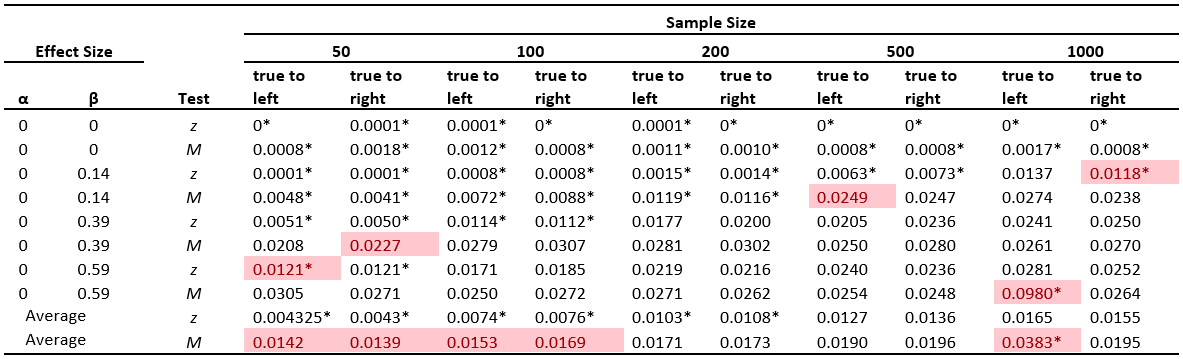
\includegraphics[width=1\linewidth]{RepliSimsTable1} \caption{Study 1 proportion of true values to left and right of 95 percent confidence intervals - zero indirect effect}\label{fig:unnamed-chunk-1}
\end{figure}

\begin{figure}
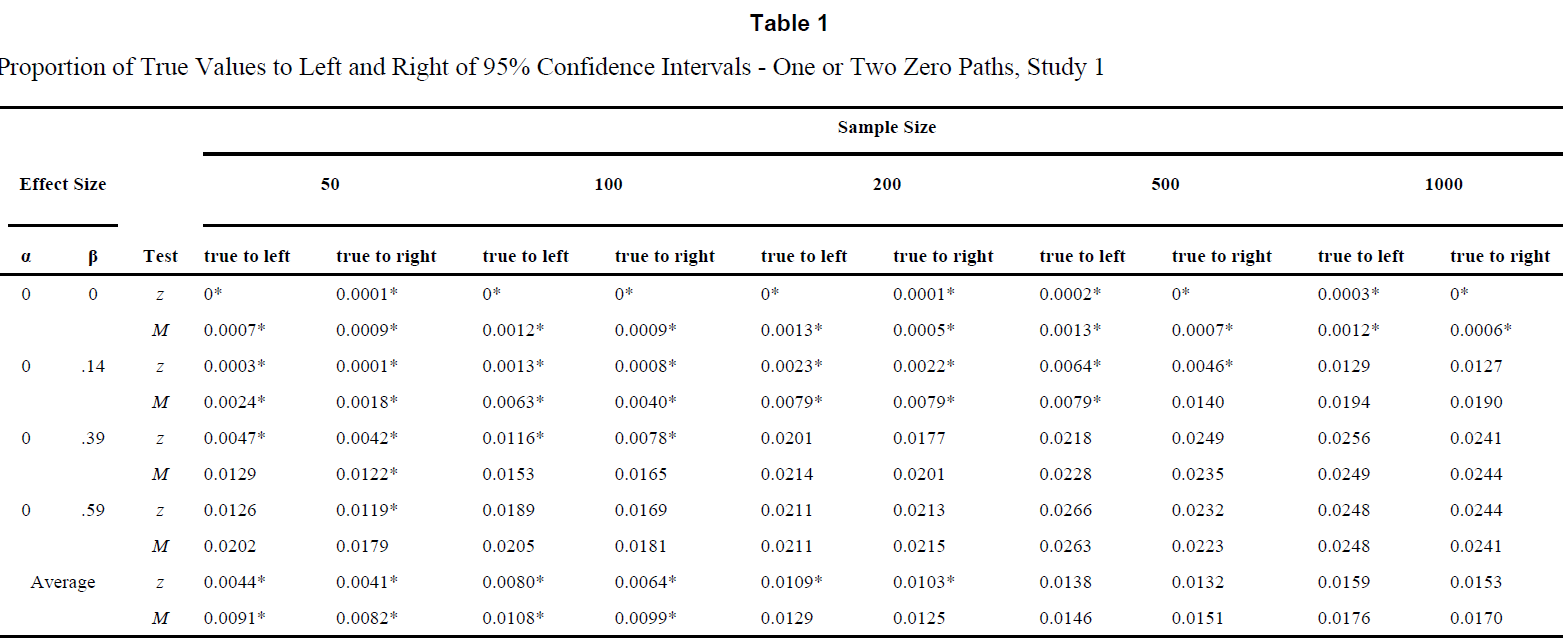
\includegraphics[width=1\linewidth]{RepliSimsMacKinnonTable1} \caption{Corresponding table from original article}\label{fig:unnamed-chunk-2}
\end{figure}

\elandscape

\newpage

\subsubsection{Table 2}

Table 2 (Figures 3 and 4 below) presents the proportion of true nonzero
indirect effects that fell to the left and right of the 95\% confidence
intervals in Study 1. The values marked in red in our replication table
indicate instances where our results disagreed with the results of the
original article, either indicating that a nonrobust proportion in the
original article was robust or that a robust proportion in the original
article was nonrobust. In total, our table disagreed with the table from
the original article 9 out of 140 times. Interestingly, six of these
nine times occurred with the \(z\) method, and only three occurred with
the \(M\) method.

\newpage

\blandscape

\begin{figure}
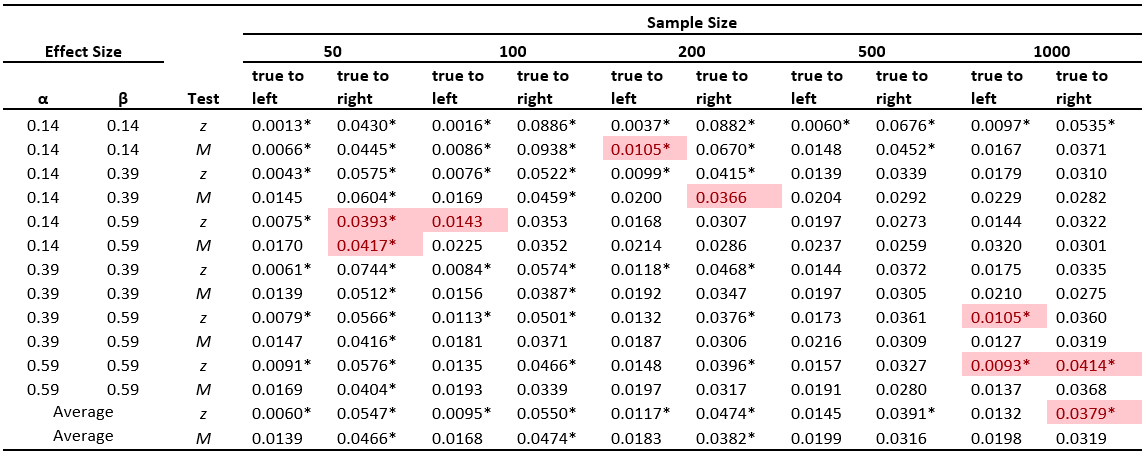
\includegraphics[width=1\linewidth]{RepliSimsTable2} \caption{Study 1 proportion of true values to left and right of 95 percent confidence intervals - nonzero indirect effect}\label{fig:unnamed-chunk-3}
\end{figure}

\begin{figure}
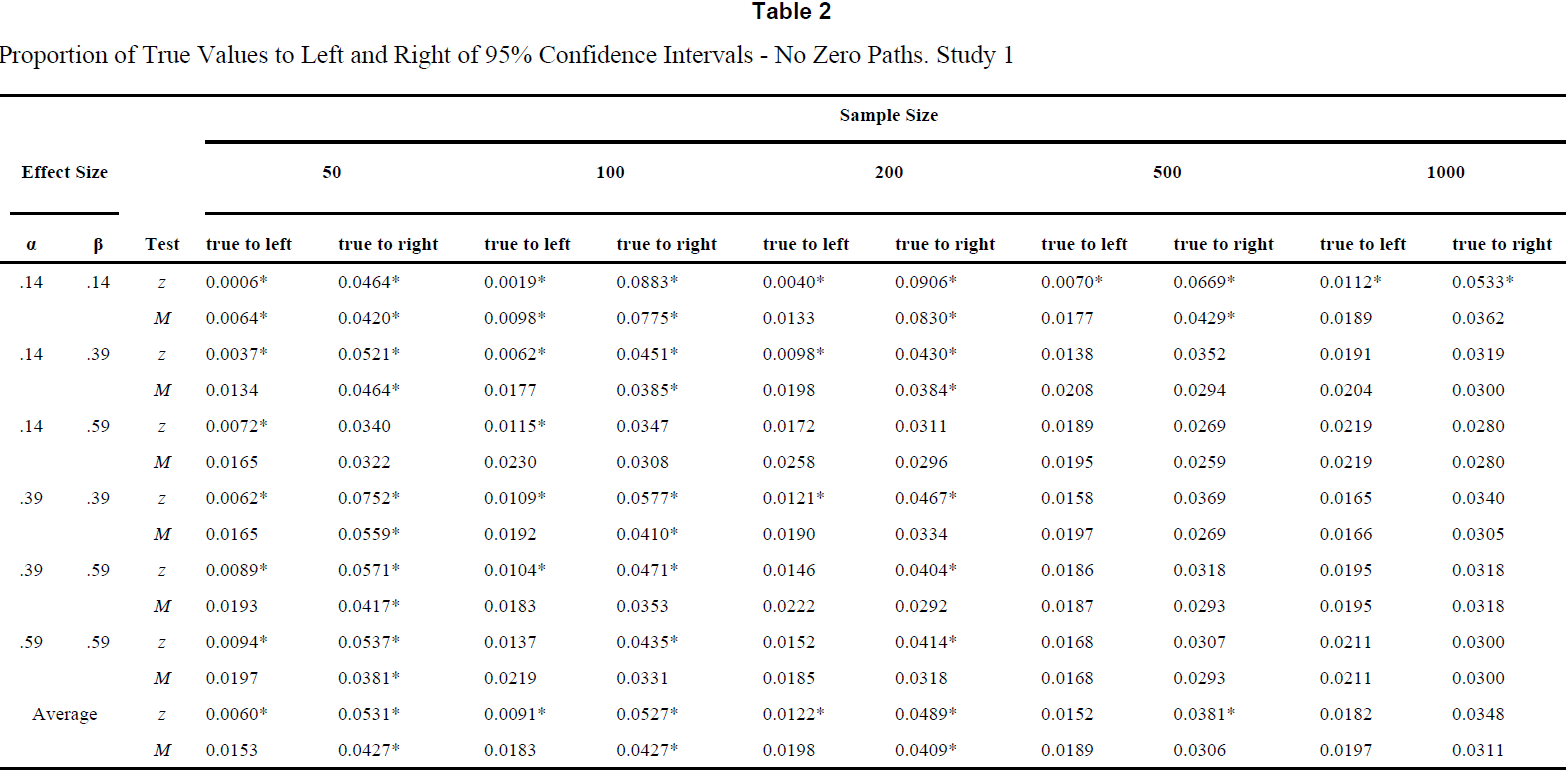
\includegraphics[width=1\linewidth]{RepliSimsMacKinnonTable2} \caption{Corresponding table from original article}\label{fig:unnamed-chunk-4}
\end{figure}

\elandscape

\newpage

\subsubsection{Table 3}

Table 3 (Figures 5 and 6 below) presents the proportion of true zero and
nonzero indirect effects that fell to the left and right of the 95\%
confidence intervals in Study 2. Results have been averaged across all
zero indirect effects (null models) and all nonzero indirect effects
(non-zero models). The values marked in red in our replication table
indicate instances where our results disagreed with the results of the
original article, either indicating that a nonrobust proportion in the
original article was robust or that a robust proportion in the original
article was nonrobust. In total, our table disagreed with the table from
the original article 25 out of 128 times. Sixteen of these 25 times
occurred with either the \(M\) method, the bootstrap-\(t\), or the
bootstrap-\(Q\), which makes sense since these methods required the most
amount of replicator degrees of freedom to implement. Recall that the
empirical-\(M\) method was not calculated in our simulation (see section
2.6 above).

\newpage

\blandscape

\begin{figure}
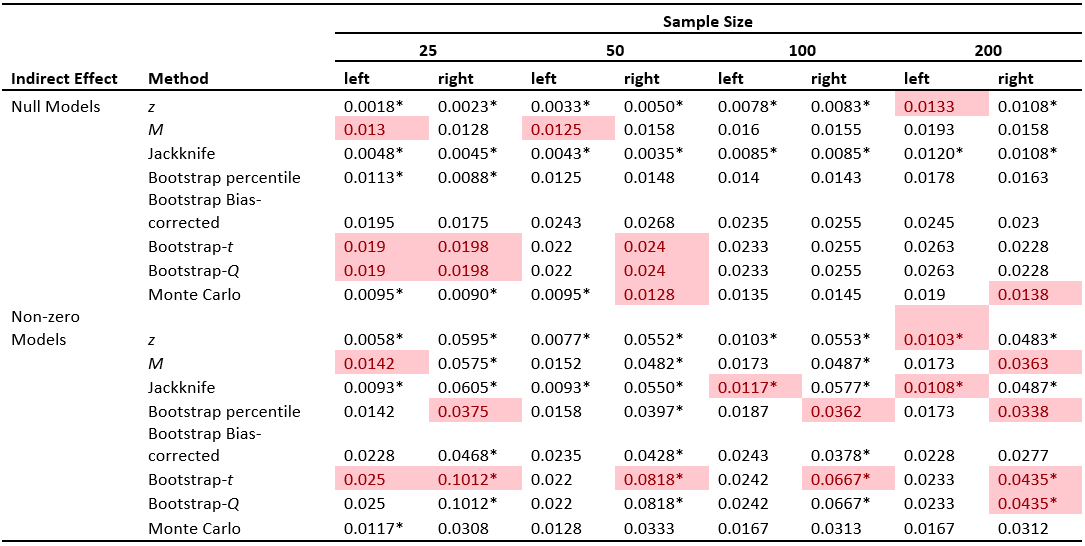
\includegraphics[width=1\linewidth]{RepliSimsTable3} \caption{Study 2 proportion of true values to left and right of 95 percent confidence intervals}\label{fig:unnamed-chunk-5}
\end{figure}

\begin{figure}
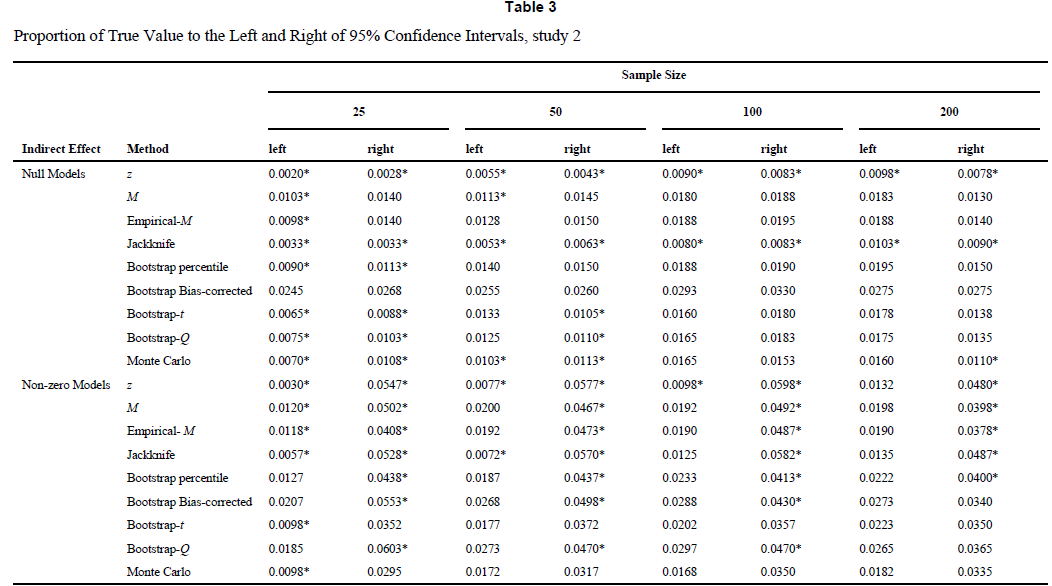
\includegraphics[width=1\linewidth]{RepliSimsMacKinnonTable3} \caption{Corresponding table from original article}\label{fig:unnamed-chunk-6}
\end{figure}

\elandscape

\newpage

\subsubsection{Table 4}

Table 4 (Figures 7 and 8 below) presents the total number of times the
proportion of true indirect effects falling to the left and right of the
confidence intervals in Study 2 was outside the robustness interval
determined by Bradley (1978). The values marked in red in our
replication table indicate instances where our results disagreed with
the results of the original article by my more than 2 for each method
and each confidence level. In total, our table disagreed with the table
from the original article by more than two 12 out of 72 times. Seven of
these 12 times occurred with either the \(M\) method, the
bootstrap-\(t\), or the bootstrap-\(Q\), which makes sense since these
methods required the most amount of replicator degrees of freedom to
implement. Recall that the empirical-\(M\) method was not calculated in
our simulation (see section 2.6 above).

\newpage

\blandscape

\begin{figure}
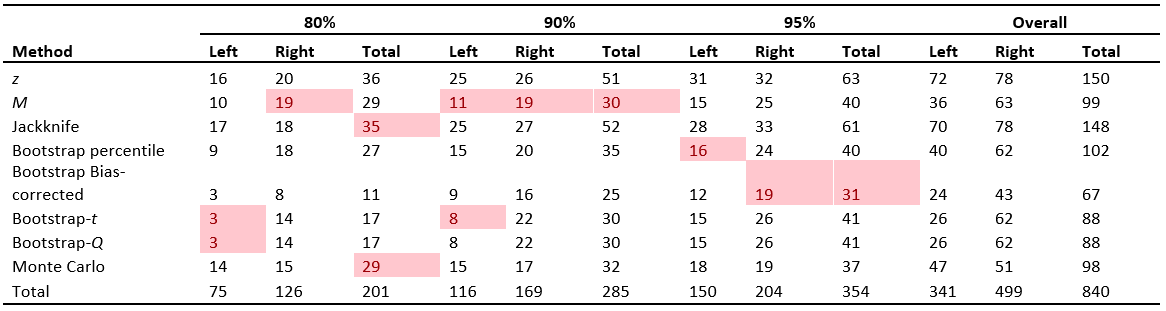
\includegraphics[width=1\linewidth]{RepliSimsTable4} \caption{Study 2 number of times proportions to left and right of CIs were outside robustness criteria}\label{fig:unnamed-chunk-7}
\end{figure}

\begin{figure}
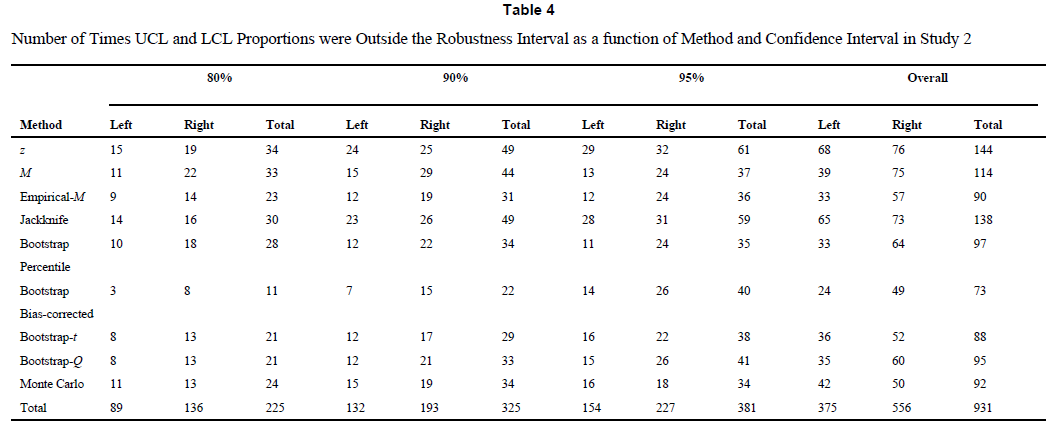
\includegraphics[width=1\linewidth]{RepliSimsMacKinnonTable4} \caption{Corresponding table from original article}\label{fig:unnamed-chunk-8}
\end{figure}

\elandscape

\newpage

\subsubsection{Table 5}

Table 5 (Figures 9 and 10 below) presents the type I error rates (null
models section) and power (non-zero models section) of the 95\%
confidence intervals in Study 2. Results have been averaged across all
zero indirect effects (null models) and all nonzero indirect effects
(non-zero models). Recall that the liberal robustness criterion given in
Bradley (1978) was used to compare type I error rates: If a type I error
rate fell outside the interval \(.5 \times \omega\) to
\(1.5 \times \omega\) (which equates to .025 to .075 for a 95\%
confidence interval), it was marked by an asterisk in the table. The
values marked in red in our replication table indicate instances where
our results disagreed with the results of the original article. For type
I error rates, this meant a rate either had an asterisk in our table
while it did not have one in the original table or it did not have one
in our table while it did in the original table. For power, this meant
power differed from the original article by more than .025. In total,
our table disagreed with the table from the original article 9 out of 64
times. All of these 9 times occurred with either the \(M\) method, the
bootstrap-\(t\), or the bootstrap-\(Q\), which makes sense since these
methods required the most amount of replicator degrees of freedom to
implement. Recall that the empirical-\(M\) method was not calculated in
our simulation (see section 2.6 above).

\newpage

\blandscape

\begin{figure}
\centering
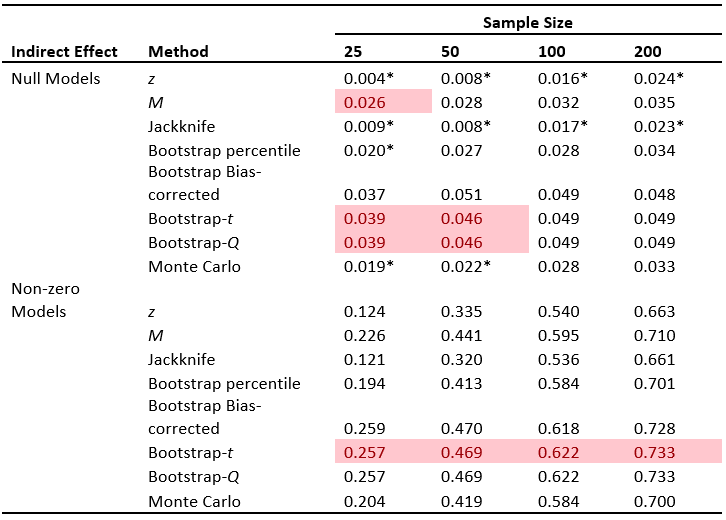
\includegraphics[width=1.00000\textwidth]{RepliSimsTable5.PNG}
\caption{Study 2 Type I Error Rates and Power}
\end{figure}

\begin{figure}
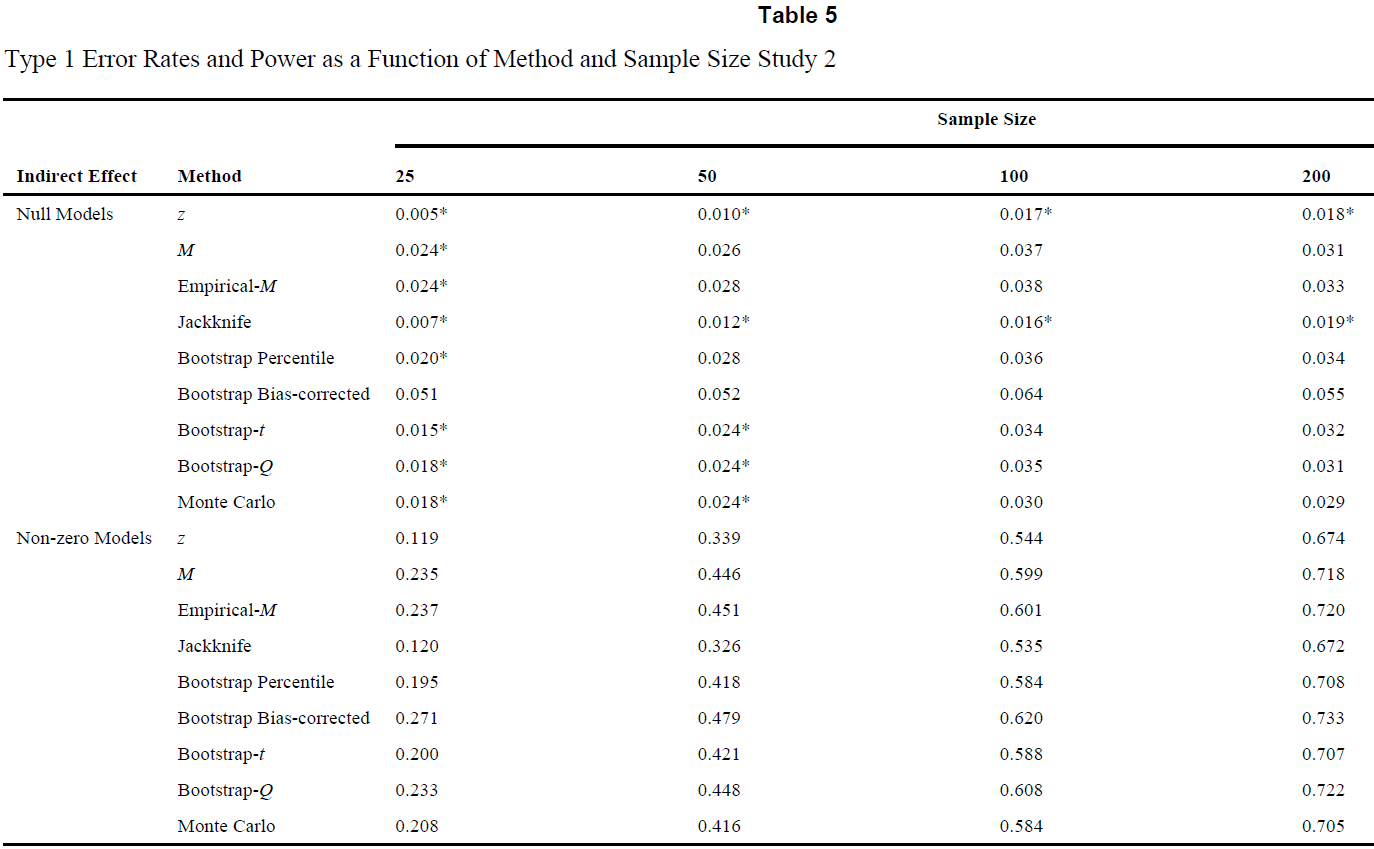
\includegraphics[width=1\linewidth]{RepliSimsMacKinnonTable5} \caption{Corresponding table from original article}\label{fig:unnamed-chunk-9}
\end{figure}

\elandscape

\newpage

\subsection{Replication of results presented in text form }

Overall, results from the text were replicated pretty well. It was
claimed in the text of the original article that, in study 1, the \(M\)
method performed better than the \(z\) method in terms of accuracy, and
we saw the same thing in our replication simulation. Similarly, in study
2, the methods were grouped into four general categories based on
performance: the \(z\) method and jackknife performed the worst; then
the percentile bootstrap, bootstrap-\(t\), and Monte Carlo method
performed better; then the \(M\) method, empirical-\(M\) method, and the
bootstrap-\(Q\) performed even better; and finally the bias-corrected
bootstrap performed the best. These general trends were seen in our
results as well, with a couple of exceptions. First, the we were not
able to produce results for the empirical-\(M\) method due to the
reasons provided in section 2.6. Also, in our study 2, the
bootstrap-\(t\) and bootstrap-\(Q\) performed the exact same in all
conditions even though they differed in performance in the original
study. This is most likely due to the replicator degrees of freedom we
had to use to implement these methods (see sections 2.7 and 2.8).

\FloatBarrier
\section{Discussion}

\subsection{Replicability}

For most of the methods, replicating the simulation was not too
difficult. The overall structure of the simulation was easy to get from
the original article, and the simulation conditions were explicitly laid
out. However, for the bootstrap-\(t\), the bootstrap-\(Q\), and
especially the \(M\) method/empirical-\(M\) method, replication proved
much more difficult. For the bootstrap-\(t\) and bootstrap-\(Q\), the
Manly (1997) book cited in the original article had to be tracked down.
For the \(M\) method/empirical-\(M\) method, the sources provided in the
original article were dead ends, and much more independent decisions had
to be made to find a way to implement them. The way we decided to go
with, using the \texttt{medci} function, was undoubtedly different from
the methods used in the original article, but no other feasible options
were found. In total, including research needed to track down sources,
around 40 hours were spent completing this replication simulation.

\subsection{Replicator degrees of freedom}

Including the code used to implement the simulation, or at least to
implement the \(M\) and empirical-\(M\) methods, would have been
immensely helpful. Without this code, it was impossible to get the
tabled critical values for the \(M\) methods integrated into our own
simulation. Also, we found that both website links provided in the paper
were either unusable or outdated and no longer provided the needed
information, so making sure that all links provided are permanent and
unchanging would be incredibly conducive to replication as well. Using
the \texttt{medci} function undoubtedly altered our results at least
somewhat. Again, as discussed in section 2.6 above, a large amount of
iterations in which the estimated \(b\) path was large had to be
discarded since the function wouldn't run, resulting in the generated
samples used in our replication simulation not truly being random.

\subsection{Equivalence of results}

With the exception of the empirical-\(M\) method being excluded and the
bootstrap-\(Q\) performing exactly the same as the bootstrap-\(t\) in
study 2, our results were quite similar to the results of the original
article and our recommendations for which methods to use would have been
similar to the original recommendations.

\section{Acknowledgments}

The replication team would like to thank Jessica Fossum for her helpful
comments on the code of our simulation.

\section{Contributions}

Authors made the following contributions according to the CRediT
framework \url{https://casrai.org/credit/}

Primary Replicator: Tristan Tibbe

\begin{itemize}
\tightlist
\item
  Data Curation\\
\item
  Formal Analysis (lead)\\
\item
  Investigation\\
\item
  Software\\
\item
  Visualization (lead)\\
\item
  Writing - Original Draft Preparation\\
\item
  Writing - Review \& Editing
\end{itemize}

Co-Pilot: Amanda Montoya

\begin{itemize}
\tightlist
\item
  Formal Analysis (supporting)\\
\item
  Investigation\\
\item
  Software (supporting)\\
\item
  Visualization (supporting)\\
\item
  Validation\\
\item
  Writing - Review \& Editing
\end{itemize}

\newpage

\section*{References}

\begingroup
\hphantom{x} \setlength{\parindent}{-0.5in} \setlength{\leftskip}{0.5in}

\hypertarget{refs}{}
\hypertarget{ref-bradley78}{}
Bradley, J. V. 1978. ``Robustness?'' \emph{British Journal of
Mathematical and Statistical Psychology} 31: 144--52.

\hypertarget{ref-mackinnon04}{}
MacKinnon, D. P., C. M. Lockwood, and J. Williams. 2004. ``Confidence
Limits for the Indirect Effect: Distribution of the Product and
Resampling Methods.'' \emph{Multivariate Behavioral Research} 39:
99--128.

\hypertarget{ref-manly97}{}
Manly, B. F. 1997. \emph{Randomization and Monte Carlo Methods in
Biology}. New York: Chapman; Hall.

\hypertarget{ref-meeker94}{}
Meeker, W. Q., and L. A. Escobar. 1994. ``An Algorithm to Compute the
Cdf of the Product of Two Normal Random Variables.''
\emph{Communications in Statistics: Simulation and Computation} 23:
271--80.

\hypertarget{ref-meeker81}{}
Meeker, W. Q., L. W. Cornwell, and L. A. Aroian. 1981. ``The Product of
Two Normally Distributed Random Variables.'' In \emph{Selected Tables in
Mathematical Statistics}, edited by W. J. Kennedy, R. E. Odeh, and J. M.
Davenport, 7th ed., 1918--27. Providence, RI: American Mathematical
Society.

\hypertarget{ref-rougier_sustainable_2017-1}{}
Rougier, Nicolas P., Konrad Hinsen, Frédéric Alexandre, Thomas Arildsen,
Lorena A. Barba, Fabien C.Y. Benureau, C. Titus Brown, et al. 2017.
``Sustainable Computational Science: The ReScience Initiative.''
\emph{PeerJ Computer Science} 3 (December): e142.
doi:\href{https://doi.org/10.7717/peerj-cs.142}{10.7717/peerj-cs.142}.

\hypertarget{ref-tofighi11}{}
Tofighi, D., and D. P. MacKinnon. 2011. ``Rmediation: A R Package for
Mediation Analysis Confidence Intervals.'' \emph{Behavior Research
Methods} 43: 692--700.
doi:\href{https://doi.org/10.3758/s13428-011-0076-x}{10.3758/s13428-011-0076-x}.

\FloatBarrier
\endgroup
\newpage

\section*{Appendix}

\subsubsection*{Reproducibility Information}

This report was last updated on 2021-09-28 00:38:58. The simulation
replication was conducted using the following computational environment
and dependencies:

\FloatBarrier

\begin{verbatim}
## - Session info ---------------------------------------------------------------
##  setting  value                       
##  version  R version 4.0.2 (2020-06-22)
##  os       Windows 8.1 x64             
##  system   x86_64, mingw32             
##  ui       RTerm                       
##  language (EN)                        
##  collate  English_United States.1252  
##  ctype    English_United States.1252  
##  tz       America/Los_Angeles         
##  date     2021-09-28                  
## 
## - Packages -------------------------------------------------------------------
##  package        * version    date       lib
##  assertthat       0.2.1      2019-03-21 [1]
##  backports        1.1.10     2020-09-15 [1]
##  blob             1.2.1      2020-01-20 [1]
##  broom            0.7.2      2020-10-20 [1]
##  callr            3.5.1      2020-10-13 [1]
##  cellranger       1.1.0      2016-07-27 [1]
##  class            7.3-17     2020-04-26 [2]
##  cli              2.1.0      2020-10-12 [1]
##  colorspace       1.4-1      2019-03-18 [1]
##  crayon           1.3.4      2017-09-16 [1]
##  DBI              1.1.0      2019-12-15 [1]
##  dbplyr           1.4.4      2020-05-27 [1]
##  desc             1.2.0      2018-05-01 [1]
##  devtools         2.3.2      2020-09-18 [1]
##  digest           0.6.25     2020-02-23 [1]
##  dplyr          * 1.0.2      2020-08-18 [1]
##  e1071          * 1.7-4      2020-10-14 [1]
##  ellipsis         0.3.1      2020-05-15 [1]
##  evaluate         0.14       2019-05-28 [1]
##  fansi            0.4.1      2020-01-08 [1]
##  forcats        * 0.5.0      2020-03-01 [1]
##  fs               1.5.0      2020-07-31 [1]
##  generics         0.0.2      2018-11-29 [1]
##  ggplot2        * 3.3.2      2020-06-19 [1]
##  glue             1.4.2      2020-08-27 [1]
##  gtable           0.3.0      2019-03-25 [1]
##  haven            2.3.1      2020-06-01 [1]
##  hms              0.5.3      2020-01-08 [1]
##  htmltools        0.5.0      2020-06-16 [1]
##  httr             1.4.2      2020-07-20 [1]
##  jsonlite         1.7.1      2020-09-07 [1]
##  knitr          * 1.30       2020-09-22 [1]
##  lavaan         * 0.6-7      2020-07-31 [1]
##  lifecycle        0.2.0      2020-03-06 [1]
##  lubridate        1.7.9      2020-06-08 [1]
##  magrittr         1.5        2014-11-22 [1]
##  MASS           * 7.3-51.6   2020-04-26 [2]
##  memoise          1.1.0      2017-04-21 [1]
##  mnormt           2.0.2      2020-09-01 [1]
##  modelr           0.1.8      2020-05-19 [1]
##  munsell          0.5.0      2018-06-12 [1]
##  pbivnorm         0.6.0      2015-01-23 [1]
##  pillar           1.4.6      2020-07-10 [1]
##  pkgbuild         1.1.0      2020-07-13 [1]
##  pkgconfig        2.0.3      2019-09-22 [1]
##  pkgload          1.1.0      2020-05-29 [1]
##  prettyunits      1.1.1      2020-01-24 [1]
##  processx         3.4.4      2020-09-03 [1]
##  ps               1.4.0      2020-10-07 [1]
##  purrr          * 0.3.4      2020-04-17 [1]
##  R6               2.5.0      2020-10-28 [1]
##  Rcpp             1.0.5      2020-07-06 [1]
##  readr          * 1.4.0      2020-10-05 [1]
##  readxl           1.3.1      2019-03-13 [1]
##  remotes          2.2.0      2020-07-21 [1]
##  RepliSimReport   0.0.0.9000 2020-11-28 [1]
##  reprex           0.3.0      2019-05-16 [1]
##  rlang            0.4.7      2020-07-09 [1]
##  rmarkdown        2.4        2020-09-30 [1]
##  RMediation     * 1.1.4      2016-03-14 [1]
##  rprojroot        2.0.2      2020-11-15 [1]
##  rstudioapi     * 0.13       2020-11-12 [1]
##  rvest            0.3.6      2020-07-25 [1]
##  scales           1.1.1      2020-05-11 [1]
##  sessioninfo      1.1.1      2018-11-05 [1]
##  stringi          1.5.3      2020-09-09 [1]
##  stringr        * 1.4.0      2019-02-10 [1]
##  testthat         2.3.2      2020-03-02 [1]
##  tibble         * 3.0.4      2020-10-12 [1]
##  tidyr          * 1.1.2      2020-08-27 [1]
##  tidyselect       1.1.0      2020-05-11 [1]
##  tidyverse      * 1.3.0      2019-11-21 [1]
##  tmvnsim          1.0-2      2016-12-15 [1]
##  usethis          1.6.3      2020-09-17 [1]
##  vctrs            0.3.4      2020-08-29 [1]
##  withr            2.3.0      2020-09-22 [1]
##  xfun             0.18       2020-09-29 [1]
##  xml2             1.3.2      2020-04-23 [1]
##  xtable         * 1.8-4      2019-04-21 [1]
##  yaml             2.2.1      2020-02-01 [1]
##  source                                   
##  CRAN (R 4.0.3)                           
##  CRAN (R 4.0.2)                           
##  CRAN (R 4.0.3)                           
##  CRAN (R 4.0.3)                           
##  CRAN (R 4.0.3)                           
##  CRAN (R 4.0.3)                           
##  CRAN (R 4.0.2)                           
##  CRAN (R 4.0.3)                           
##  CRAN (R 4.0.3)                           
##  CRAN (R 4.0.3)                           
##  CRAN (R 4.0.3)                           
##  CRAN (R 4.0.3)                           
##  CRAN (R 4.0.3)                           
##  CRAN (R 4.0.3)                           
##  CRAN (R 4.0.2)                           
##  CRAN (R 4.0.3)                           
##  CRAN (R 4.0.3)                           
##  CRAN (R 4.0.3)                           
##  CRAN (R 4.0.2)                           
##  CRAN (R 4.0.3)                           
##  CRAN (R 4.0.3)                           
##  CRAN (R 4.0.3)                           
##  CRAN (R 4.0.3)                           
##  CRAN (R 4.0.3)                           
##  CRAN (R 4.0.2)                           
##  CRAN (R 4.0.3)                           
##  CRAN (R 4.0.3)                           
##  CRAN (R 4.0.3)                           
##  CRAN (R 4.0.2)                           
##  CRAN (R 4.0.3)                           
##  CRAN (R 4.0.2)                           
##  CRAN (R 4.0.2)                           
##  CRAN (R 4.0.3)                           
##  CRAN (R 4.0.3)                           
##  CRAN (R 4.0.3)                           
##  CRAN (R 4.0.2)                           
##  CRAN (R 4.0.2)                           
##  CRAN (R 4.0.3)                           
##  CRAN (R 4.0.3)                           
##  CRAN (R 4.0.3)                           
##  CRAN (R 4.0.3)                           
##  CRAN (R 4.0.3)                           
##  CRAN (R 4.0.3)                           
##  CRAN (R 4.0.3)                           
##  CRAN (R 4.0.3)                           
##  CRAN (R 4.0.3)                           
##  CRAN (R 4.0.3)                           
##  CRAN (R 4.0.3)                           
##  CRAN (R 4.0.3)                           
##  CRAN (R 4.0.3)                           
##  CRAN (R 4.0.2)                           
##  CRAN (R 4.0.2)                           
##  CRAN (R 4.0.3)                           
##  CRAN (R 4.0.3)                           
##  CRAN (R 4.0.3)                           
##  Github (replisims/RepliSimReport@0cf1ce2)
##  CRAN (R 4.0.3)                           
##  CRAN (R 4.0.2)                           
##  CRAN (R 4.0.2)                           
##  CRAN (R 4.0.3)                           
##  CRAN (R 4.0.3)                           
##  CRAN (R 4.0.5)                           
##  CRAN (R 4.0.3)                           
##  CRAN (R 4.0.3)                           
##  CRAN (R 4.0.3)                           
##  CRAN (R 4.0.2)                           
##  CRAN (R 4.0.2)                           
##  CRAN (R 4.0.3)                           
##  CRAN (R 4.0.3)                           
##  CRAN (R 4.0.3)                           
##  CRAN (R 4.0.3)                           
##  CRAN (R 4.0.3)                           
##  CRAN (R 4.0.3)                           
##  CRAN (R 4.0.3)                           
##  CRAN (R 4.0.3)                           
##  CRAN (R 4.0.3)                           
##  CRAN (R 4.0.2)                           
##  CRAN (R 4.0.3)                           
##  CRAN (R 4.0.3)                           
##  CRAN (R 4.0.2)                           
## 
## [1] C:/Users/tdtibbet/Documents/R/win-library/4.0
## [2] C:/Program Files/R/R-4.0.2/library
\end{verbatim}


\end{document}
